% !TeX root = ../../../../thesis.tex

\subsection{DC}
\label{subsec:dc-testbed-eval}

The DC testbed has six LEDs, as explained in \autoref{subsec:dc-testbed}.
Therefor six Gold codes will be used.
From \autoref{tbl:correlation-gold-families}, we can see that for $m = 6$, where $m$ is the number of simultaneous transmitters such that no destructive interference takes place, requires a code length of 511 or higher.
With the DC testbed the experiments have been performed with a constant modulation frequency of 1 kHz.
Every two successive samples are $\frac{1}{1000} = 1$ ms apart.

In \autoref{fig:raw-dc-testbed-adc-data-n=9} the raw ADC from the DC testbed can be seen.
The left y-axis represents the raw ADC data and the right y-axis is converted to current.
Six LEDs are simultaneous continuously modulating with different starting times.
From the figure, seven horizontal lines can be seen.
Each line represents how many LEDs are on, none through six.
This raw data is already in a form for which we can start calculating the correlation with a Gold sequence, no additional signal processing is needed.

In \autoref{fig:correlation-dc-testbed-n=9}, the correlation for one Gold sequence can be seen, which is also one of the sequences used to modulate an LED and the correlation for another Gold sequence can be seen, which is not part of the sequences used to modulate any LED.
All the correlation results stay below the threshold (See \autoref{eq:T}) except for the noticeable peaks.
These peaks occur when the correlation is calculated when there is no time shift as already shown in \autoref{fig:autocorr-gold}.

Since all the correlation levels are below the threshold, and the peaks are above the threshold, every result is correct.
There are only true positives and true negatives.
So the F-measure is equal to $1$ according \autoref{eq:F-measure}.
This can also be seen in \autoref{fig:f-measure-dc-testbed-n=9}.

\begin{figure}[!tbp]
  \centering
  \begin{minipage}[b]{0.49\textwidth}
    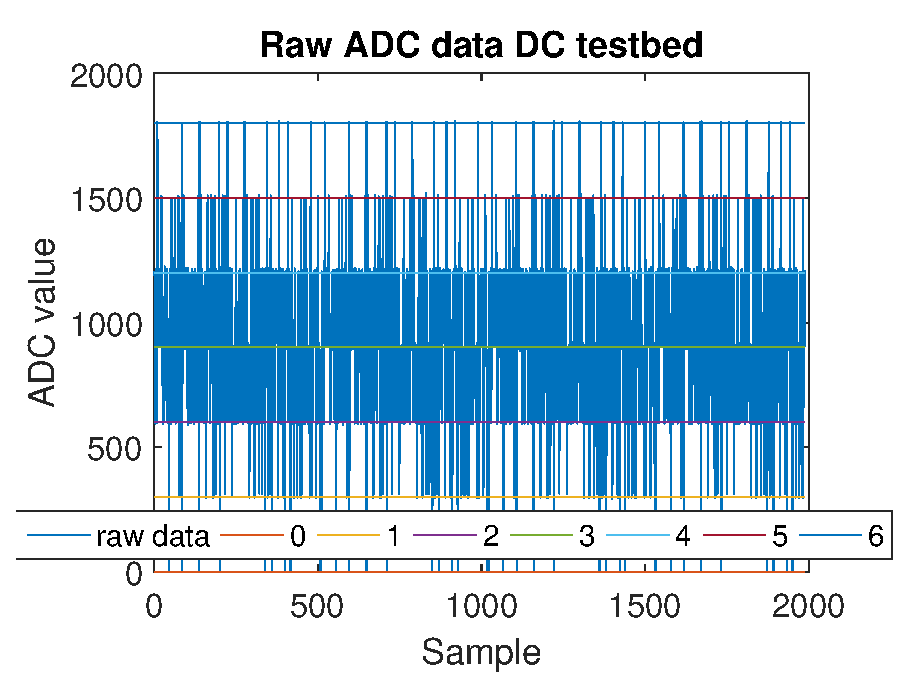
\includegraphics[width=\textwidth]{chapters/evaluation-chapters/hardware/dc/raw-dc-testbed-adc-data-n=9.eps}
    \caption{Raw ADC data from the DC testbed. With seven distinguishable entries, following the on-state of the combinations of LEDs. With a sequence length of 511.}
	\label{fig:raw-dc-testbed-adc-data-n=9}
  \end{minipage}
  \hfill
  \begin{minipage}[b]{0.49\textwidth}
    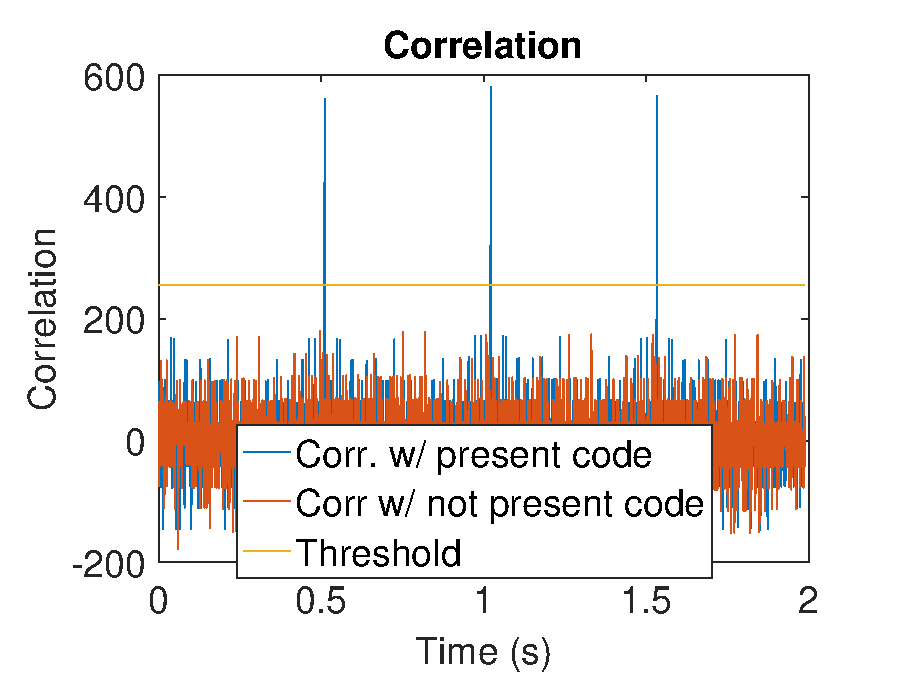
\includegraphics[width=\textwidth]{chapters/evaluation-chapters/hardware/dc/correlation-dc-testbed-n=9.eps}
    \caption{Correlations results from Gold sequences which are and which are not present, with the decision threshold. With a sequence length of 511.}
	\label{fig:correlation-dc-testbed-n=9}
  \end{minipage}
\end{figure}

To show how the F-measure would behave when there are false positives and/or false negatives a different Gold set is chosen.
A length of 127 is chosen, since it may only have three simultaneous continuously modulating LEDs (\autoref{tbl:correlation-gold-families}).
Again the six LEDs are simultaneous continuously modulating with different starting times.
For which the raw ADC can be seen in \autoref{fig:raw-dc-testbed-adc-data-n=7} on the left y-axis and on the right y-axis the current.
And the correlation can be found in \autoref{fig:correlation-dc-testbed-n=7}.
In the correlation figure, peaks can be seen that cross the threshold line, which are the autocorrelation peaks of the sequence.
They are supposed to be there.
But also other results can be seen to cross the threshold line.
These are the false positives, they occur because this code length can not support this much simultaneous transmitters.
The F-measure for these correlation results can be found in \autoref{fig:f-measure-dc-testbed-n=7}.


\begin{figure}[!tbp]
  \centering
  \begin{minipage}[b]{0.49\textwidth}
    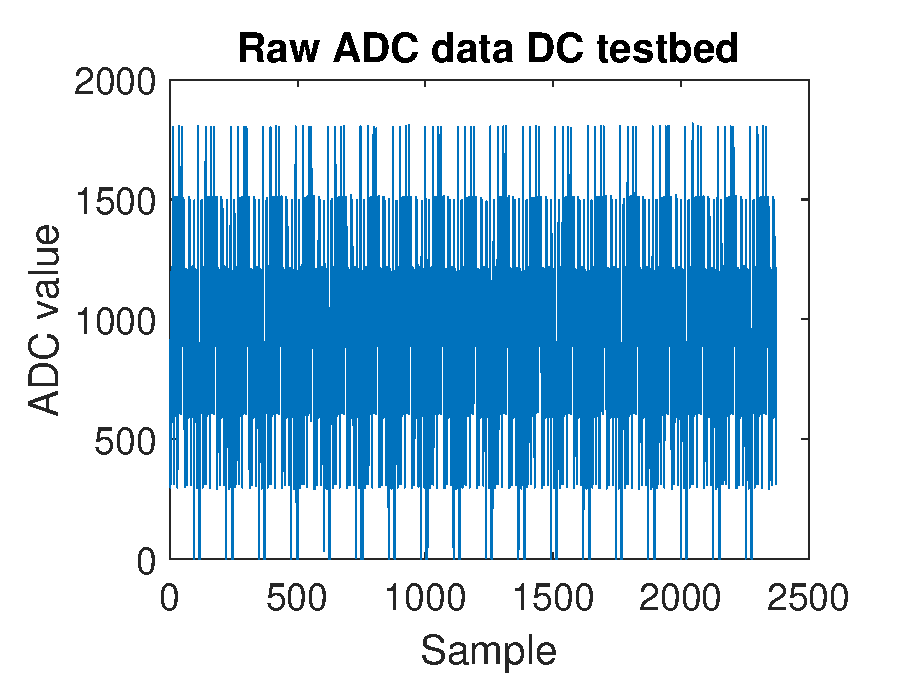
\includegraphics[width=\textwidth]{chapters/evaluation-chapters/hardware/dc/raw-dc-testbed-adc-data-n=7.eps}
    \caption{Raw ADC data from the DC testbed. With seven distinguishable entries, following the on-state of the combinations of LEDs. With a sequence length of 127  on the DC testbed.}
	\label{fig:raw-dc-testbed-adc-data-n=7}
  \end{minipage}
  \hfill
  \begin{minipage}[b]{0.49\textwidth}
    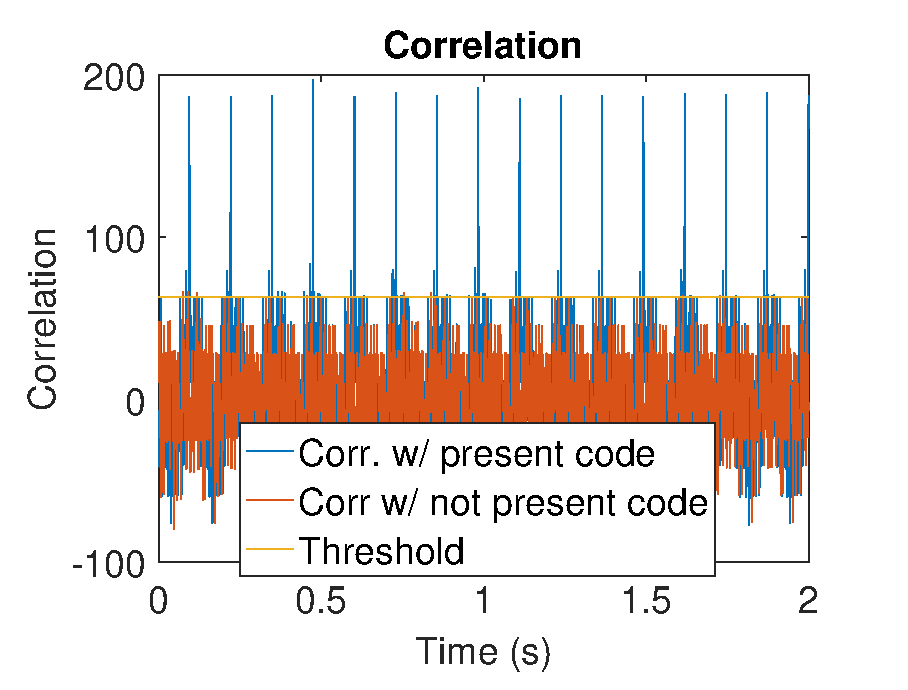
\includegraphics[width=\textwidth]{chapters/evaluation-chapters/hardware/dc/correlation-dc-testbed-n=7.eps}
    \caption{Correlations results from Gold sequences which are and which are not present, with the decision threshold. With a sequence length of 127 on the DC testbed.}
	\label{fig:correlation-dc-testbed-n=7}
  \end{minipage}
\end{figure}


\begin{figure}[!tbp]
  \centering
  \begin{minipage}[b]{0.49\textwidth}
    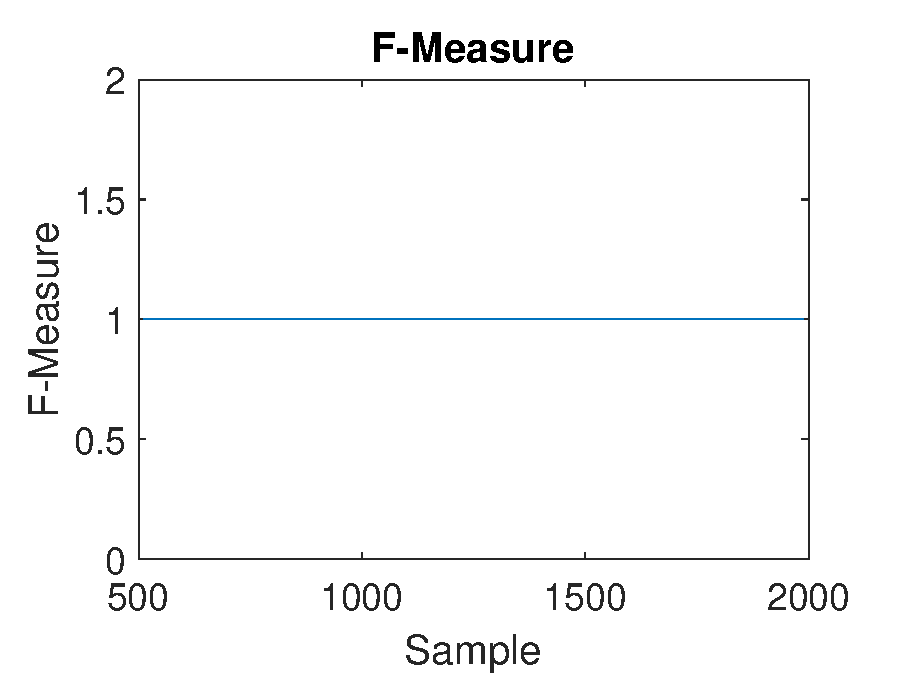
\includegraphics[width=\textwidth]{chapters/evaluation-chapters/hardware/dc/f-measure-dc-testbed-n=9.eps}
	\caption{F-Measure of DC testbed correlation (\autoref{fig:correlation-dc-testbed-n=9}), with sequence length of 511.}
	\label{fig:f-measure-dc-testbed-n=9}
  \end{minipage}
  \hfill
  \begin{minipage}[b]{0.49\textwidth}
	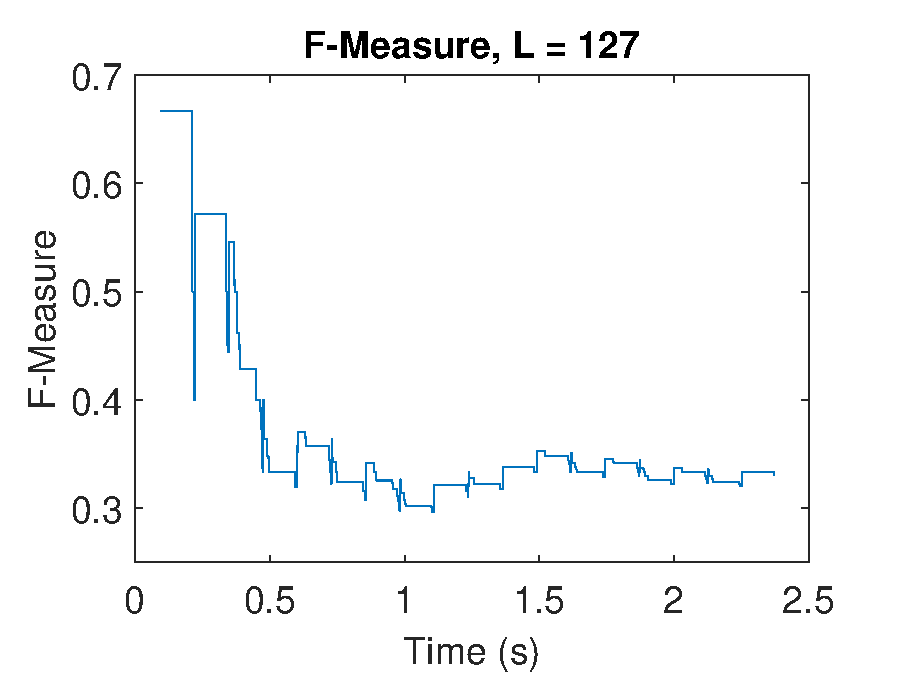
\includegraphics[width=\textwidth]{chapters/evaluation-chapters/hardware/dc/f-measure-dc-testbed-n=7.eps}
	\caption{F-Measure of DC testbed correlation (\autoref{fig:correlation-dc-testbed-n=7}), with sequence length of 127.}
	\label{fig:f-measure-dc-testbed-n=7}
  \end{minipage}
\end{figure}